% ICASSP 2027 manuscript, using the supplied Template.tex and spconf.sty.
% Canonical source; paper_draft_icassp/main.tex is a build-time delivery copy.
\documentclass{article}
\usepackage{spconf,amsmath,amssymb,graphicx,booktabs}
\usepackage[hidelinks]{hyperref}
\title{Not All Changes Matter:\\Decision-Aligned Delta Selection for Speech Recognition}
\name{\fontsize{10}{10}\selectfont Mingjun Yang\quad Chaofan Yang\quad Jiahao Zhao\quad Bo Zhang}
\address{School of Artificial Intelligence, Optics and Electronics (iOPEN)\\
Northwestern Polytechnical University, Xi'an 710072, China}
\newcommand{\CTC}{\mathrm{CTC}}
\newcommand{\Du}{\mathcal{D}_{u}}
\begin{document}
\ninept
\maketitle

\begin{abstract}
Recent studies improve speech recognition adaptation by incorporating pretrained-to-fine-tuned representation shifts with other features, but treat these changes as a whole. Whether adapted recognizers rely on all shift coordinates remains underexplored. We propose \textbf{Decision-Aligned Delta Selection (DADS)}, a task-aware framework that identifies decision-supporting representation shifts by aligning feature changes with the adapted recognizer's decision sensitivity. We find that adaptation gains are concentrated in a subset of fine-tuning-induced representation shifts in the encoder's native output basis, rather than uniformly distributed across coordinates. A released L2-ARCTIC recognizer maintains nearly full accuracy after discarding 25\% of shifts (10.58\% vs. 10.50\% WER), and DADS preserves substantially more performance than magnitude selection when retaining only half of the shifts (11.71\% vs. 16.64\% WER). Further reversion analyses show that the adapted recognizer relies unevenly on the induced shifts.
\end{abstract}

\begin{keywords}
speech recognition, self-supervised learning, model adaptation, representation analysis, feature selection
\end{keywords}

\section{Introduction}
\label{sec:intro}
Modern speech recognition systems increasingly rely on large-scale self-supervised speech representations, which provide strong initialization for adapting models to new speakers, accents, and domains~\cite{mohamed2022review,baevski2020wav2vec,hsu2021hubert,chen2022wavlm,baevski2022data2vec,yang2021superb}. Through supervised fine-tuning, these models acquire task-specific capabilities from limited labeled speech and achieve substantial improvements under distribution shifts~\cite{thai2026contrastive,hu2022lora,bagat2025maslora}. Adaptation reshapes the learned representation space by introducing substantial differences between pretrained and adapted representations, yet how such information is organized within the representation space remains poorly understood.

Recent studies have demonstrated that differences between pretrained and adapted models contain transferable information. Task arithmetic transfers model behaviors through parameter differences, while TIES-Merging and DARE selectively manipulate such differences for model combination~\cite{ilharco2023task,yadav2023ties,yu2024dare}. Similar ideas have also been explored in automatic speech recognition through task vector algebra and selective model merging~\cite{ramesh2024taskvector,shankar2025selective}. In representation space, \emph{Mind the Shift} exploits delta embeddings, defined as the difference between pretrained and fine-tuned speech representations, to enhance child ASR; accent steering further utilizes representation differences between speech groups to control adaptation behavior~\cite{wang2026mind,sun2026activation}.

% Queue the wide method figure for the next page.
\begin{figure*}[t]
\centering

\includegraphics[width=\textwidth]{figures/dads_overview1_01(1).png}
\caption{Overview of DADS. (a) Shift $\Delta$ is combined with CTC sensitivity $G=\partial\ell/\partial E_a$ from the frozen adapted head. Averaging absolute elementwise products over valid training frames gives a global top-$K$ native-coordinate mask. (b) Selected coordinates keep adapted values; others restore reference values. The same frozen head decodes without retraining. Labels and gradients are calibration-only; feature strips schematically show corresponding coordinates.}
\label{fig:overview}
\end{figure*}

Although existing methods vary in how representation differences are constructed and utilized, they generally treat representation shifts as a unified adaptation signal without considering how individual changes affect the adapted recognizer. Our key insight is that shift relevance changes across the representation-to-decision boundary: from feature movement in the representation space to decision sensitivity in the adapted recognizer. A large shift may have limited impact if the recognizer is insensitive to that direction, while a smaller shift can be critical when aligned with a decision-sensitive direction.

Two observations support this decision-aligned view. First, fine-tuning-induced shifts exhibit highly non-uniform utility across native output coordinates. Under a fixed retention budget, preserving selected shifts can maintain adaptation performance, while removing different groups of the same size leads to substantially different recognition outcomes. Second, shift magnitude alone cannot explain adaptation utility. Useful shifts emerge from the interaction between representation movement and the recognizer's decision sensitivity, rather than from either factor independently.

Based on these observations, we propose \textbf{Decision-Aligned Delta Selection (DADS)}, a decision-aligned pruning framework for fine-tuning-induced representation shifts. DADS first decomposes adaptation into native output coordinates and evaluates each coordinate by measuring how its change affects the adapted CTC decision. Specifically, DADS combines shift magnitude with CTC objective sensitivity to identify decision-supporting shifts, then selectively retains informative changes while removing redundant adaptation signals. The intervention keeps the adapted CTC head and decoding fixed, so retention and reversion directly test which changes are sufficient and necessary for the existing recognizer (Fig.~\ref{fig:overview}).

We evaluate DADS on L2-ARCTIC across adapted ASR models~\cite{zhao2018l2arctic} and reveal substantial redundancy in fine-tuning-induced shifts. DADS retains 98.8\% of the full adaptation gain using only 50\% of native output coordinates, achieving 11.71\% WER compared with 16.64\% for magnitude-based selection. Counterfactual reversion further shows that high-utility shift groups are more decision-relevant, causing substantially larger degradation when removed than low-utility groups.

Our main contributions are summarized as follows:
\begin{enumerate}
\setlength{\itemsep}{2pt}
\setlength{\parsep}{0pt}
\item We identify that adaptation utility is concentrated in a decision-dependent subset of native-coordinate fine-tuning shifts, showing why shift magnitude alone is insufficient.
\item We align representation displacement with adapted CTC sensitivity to select decision-supporting native-coordinate shifts and remove redundant changes without retraining.
\item We use frozen-head retention and reversion to establish which shifts the adapted recognizer functionally relies on and to verify the value of decision-aligned selection.
\end{enumerate}



\section{Decision-Aligned Delta Selection}
\label{sec:method}

\subsection{Native-coordinate shift selection}
\label{sec:native_frame}
DADS treats fine-tuning as a shift at the final encoder--CTC interface. It has two steps: (1) score each native coordinate by its movement and adapted CTC sensitivity; and (2) retain the highest-scoring changes while restoring the remainder to the reference representation. The adapted head is fixed after fine-tuning.

\textbf{Learned native frame.} We call the channel basis of the final encoder representation the native frame, i.e., the learned computational interface exposed to the adapted recognition head. Let $h=E(x)$ and $z=Wh+b$. For any orthogonal matrix $Q$, the equivalent parameterization
\begin{equation}
 h'=Qh, \qquad W'=WQ^\top
 \label{eq:orthogonal_interface}
\end{equation}
preserves the input--output computation because $W'h'+b=Wh+b$, while a change is expressed as $\Delta h'=Q\Delta h$. The basis control in Section~\ref{sec:reparam} tests whether DADS concentration follows the learned frame used by the trained recognizer. The frame is shaped jointly by the fine-tuned encoder and its readout; a learned input projection in a nonlinear decoder can absorb the same basis change before subsequent nonlinear operations.


\subsection{Frozen-head intervention}
As shown in Fig.~\ref{fig:overview}, the reference and adapted encoders map utterance $x$ to final-layer features $E_r(x),E_a(x)\in\mathbb{R}^{T_x\times d}$, where $T_x$ is the number of output frames and $d$ is the number of native coordinates. Their difference is
\begin{equation}
 \Delta(x)=E_a(x)-E_r(x).
 \label{eq:shift}
\end{equation}
Both encoders receive the same waveform and have the same frame resolution. When the reference is the recorded initialization, $\Delta$ is the change induced by fine-tuning. We also apply the operation to a released recognizer and a separately obtained reference, as specified in Section~\ref{sec:setup}.

A binary mask $m\in\{0,1\}^{d}$ retains $K$ native coordinates of the change:
\begin{equation}
 \widetilde E_m(x)=E_r(x)+m\odot\Delta(x).
 \label{eq:mask}
\end{equation}
The mask is broadcast over frames and shared across utterances. Keeping every change gives the complete adapted representation (\emph{Full}); keeping none gives the reference representation (\emph{NoShift}).

Every condition uses the adapted affine CTC head $g_a(h)=W_ah+b_a$ and greedy decoding. NoShift therefore sends reference features through this same head. This comparison asks what the \emph{adapted recognizer} needs from its feature changes. Because neither the encoder nor the head is retrained after masking, a WER difference directly records the effect of substituting the selected features. All masks are defined in the learned native final-layer frame exposed to $W_a$, which is kept fixed across models, budgets, and interventions.

The effect of a feature change therefore depends on how the recognition head uses its coordinate, motivating a score based on the recognition loss rather than shift magnitude alone.

\subsection{Decision-aligned scoring}
On a labeled subset $\Du$ of the adaptation training data, we compute the loss at the complete adapted features:
\begin{equation}
 \ell_{x,y}=\frac{1}{|y|}\mathcal{L}_{\CTC}\bigl(g_a(E_a(x)),y\bigr),
 \label{eq:loss}
\end{equation}
where $|y|$ is the transcript length in characters. CTC sums over valid frame-to-label alignments~\cite{graves2006ctc}; no forced alignment is required for this score. The length normalization gives each utterance a loss per target character.

Undoing a change in native coordinate $i$ perturbs each frame by $-\Delta_{t,i}$. In a first-order approximation, its effect on the loss involves the product of the change and the corresponding gradient. Following Taylor saliency~\cite{molchanov2017pruning}, DADS aggregates the absolute products:
\begin{equation}
 U_i=\frac{1}{N_u}\sum_{(x,y)\in\Du}\sum_{t=1}^{T_x}
 \left|\Delta_{t,i}(x)\frac{\partial\ell_{x,y}}{\partial E_{a,t,i}}\right|,
 \label{eq:utility}
\end{equation}
where $N_u=\sum_{(x,y)\in\Du}T_x$. We take the absolute value at each frame before averaging, so positive and negative products do not cancel. Only valid frames contribute. The result is one score per native output coordinate, computed from a single pass through cached features and the fixed head.

DADS keeps the $K$ native coordinates with the largest $U_i$. The score is high when a coordinate both moves during adaptation and affects the adapted recognition loss.

For comparison, \emph{Magnitude} replaces the product in Eq.~\eqref{eq:utility} with $|\Delta_{t,i}|$, while \emph{Gradient} uses $|\partial\ell_{x,y}/\partial E_{a,t,i}|$. Both use the same valid-frame average and retain the same number of coordinates. \emph{Random} selects exactly $K$ coordinates uniformly. We also undo the highest- or lowest-scoring quarter to test the necessity of the ranking.

\section{Experimental Setup}
\label{sec:setup}
\subsection{Datasets}
We evaluate DADS on L2-ARCTIC~\cite{zhao2018l2arctic} using the speaker-disjoint splits released by Thai et al.~\cite{thai2026contrastive}. Each split uses 18 speakers for training and development and holds out six speakers for testing, covering the same six first-language groups. Folds~0--2 contain 16,312, 16,070, and 15,953 training utterances, respectively; their development sets contain 1,867, 1,979, and 2,086 utterances, and their test sets contain 675, 686, and 691 utterances. This design lets us ask whether a ranking computed from training speech transfers to unseen speakers within the same accent groups.

\subsection{Adapted models}
We use four adapted recognizers to answer two complementary questions: whether DADS works for a released model and whether the same selection principle transfers across controlled fine-tuning runs. The released wav2vec~2.0 Large recognizer is adapted to Fold~0 with CTC and supervised contrastive learning~\cite{khosla2020supcon,thai2026contrastive}. We refer to this condition as \emph{Rel-W2V2-F0}; its reference is the LibriSpeech-960h wav2vec~2.0 Large checkpoint~\cite{panayotov2015librispeech}. Because the released model and reference differ in feature-extractor normalization, this condition tests selection between a released recognizer and a separately obtained reference in the learned native final-layer frame.

For controlled comparisons, wav2vec~2.0 Large is adapted on Folds~1/2 with CTC and supervised contrastive learning, and data2vec Audio Large is adapted on Fold~0 with CTC. We refer to these conditions as \emph{W2V2-F1}, \emph{W2V2-F2}, and \emph{D2V-F0}, respectively. Their references are the recorded initializations, so the corresponding representation differences measure changes induced by fine-tuning. Both source models have 960~h of LibriSpeech ASR supervision. All final-layer features have dimension $d=1024$, and every adapted head predicts 32 output symbols.

During adaptation, we warm up the head for one epoch at learning rate $3\times10^{-6}$ and then jointly train at $10^{-5}$ with frozen convolutional features. Development WER selects the checkpoint within a 40-epoch budget. W2V2-F1/F2 use two GPUs, batch size 24 per GPU, a linear schedule, contrastive weight 0.05, temperature 0.1, and projection dimension 256. D2V-F0 uses batch size four on one GPU and a cosine schedule. Each model comes from one adaptation run with seed 1337.

\subsection{Calibration and evaluation}
DADS obtains one global ranking of native-coordinate changes from labeled adaptation speech. We select every tenth training utterance after sorting identifiers within each speaker, giving 1,640/1,615/1,600 calibration utterances for Folds~0/1/2. These utterances remain part of adaptation training, but their labels are used only to determine the ranking; development and test utterances are not used for coordinate scoring. The ranking is therefore defined from training speech before evaluation on held-out speakers.

To keep the comparison focused on the selection rule, all methods use the same adapted model, reference, head, and retained coordinate count. Final-layer features are cached in float32 from the same 16-kHz waveforms. After a ranking is computed, each condition only composes the selected features and applies the fixed adapted head. All conditions use complete utterances and greedy CTC decoding without a language model. WER is the total word edit distance divided by the total reference word count.

We report retention budgets of 25\%, 50\%, and 75\% where available, and compare removal of the highest- and lowest-scoring quarters at 25\%. Random results use mask seeds 1337, 2027, and 31415 and are reported as the mean and sample standard deviation over masks of the same model. For Rel-W2V2-F0, we compute paired intervals from 10,000 utterance-bootstrap samples of the existing predictions.

We therefore ask, in order: can DADS preserve recognition; does it beat matched controls; which shifts are necessary; and do native-frame and calibration analyses explain its behavior?

\section{Results}
\label{sec:results}
\subsection{Can DADS preserve recognition with fewer changes?}
\label{sec:retention}
We first test the central sufficiency question: how much recognition is preserved when only a fixed fraction of the representation shift is retained? Table~\ref{tab:retention} summarizes the main retention comparison across the released and controlled conditions.

\begin{table}[!h]
\centering
\caption{Test WER (\%) after retaining selected changes. Rel.-F0 is the released wav2vec~2.0 condition; W2V2-F1/F2 and D2V-F0 are controlled conditions. Full and NoShift retain all and none of the changes, respectively.}
\label{tab:retention}
\begin{tabular}{@{}lrrrr@{}}
\toprule
Selection & Rel.-F0 & W2V2-F1 & W2V2-F2 & D2V-F0\\
\midrule
Full & 10.50 & 15.14 & 14.46 & 11.39\\
DADS, 75\% & 10.58 & 15.36 & 14.54 & 10.96\\
DADS, 50\% & 11.71 & 16.01 & 15.58 & 12.94\\
Magnitude, 50\% & 16.64 & 16.63 & 16.48 & 13.75\\
NoShift & 118.91 & 20.33 & 19.15 & 13.77\\
\bottomrule
\end{tabular}

\end{table}

For Rel-W2V2-F0, DADS retains 75\% of the changes at 10.58\% WER, close to 10.50\% for Full. The difference is 0.09 percentage points, with a paired 95\% interval of $[-0.21,0.38]$. At 50\%, DADS gives 11.71\%, compared with 16.64\% for Magnitude: a 29.6\% relative WER reduction. The paired difference is $-4.92$ points, with interval $[-5.72,-4.16]$.

The pattern transfers to the controlled models. At 50\%, DADS improves over Magnitude by 0.62/0.91/0.80 points for W2V2-F1/W2V2-F2/D2V-F0. At 75\%, W2V2-F1/F2 are within 0.22/0.08 points of Full and D2V-F0 reaches 10.96\%; Full beats NoShift throughout. Thus, much of the adaptation change can be restored with little loss.

\subsection{Do decision-aligned scores improve selection?}
\label{sec:controls}
The retention results establish that DADS can preserve recognition, but not whether the gain comes from decision alignment or merely from selecting a subset of coordinates. We therefore compare the rules at the same 50\% budget in Table~\ref{tab:sourcecontrols}.

\begin{table}[t]
\centering
\caption{W2V2-F1/F2 test WER (\%) at 50\% retention. Random results are mean $\pm$ SD over three masks. Bold marks the lowest mean WER in each column.}
\label{tab:sourcecontrols}
\setlength{\tabcolsep}{4pt}
\begin{tabular}{@{}lrr@{}}
\toprule
Method & W2V2-F1 & W2V2-F2\\
\midrule
DADS & 16.01 & 15.58\\
Magnitude & 16.63 & 16.48\\
Gradient & 19.79 & 20.48\\
Random & $23.39\pm0.58$ & $24.20\pm0.81$\\
\bottomrule
\end{tabular}

\end{table}

At 50\%, DADS lowers WER relative to Magnitude, Gradient, and Random in both W2V2-F1 and W2V2-F2.

\subsection{Which changes does the adapted recognizer rely on?}
\label{sec:reversion}
Retention tests sufficiency; we next test necessity by reverting groups of the same size. With a fixed quarter reversion (Fig.~\ref{fig:deletion}), undoing the highest-scoring coordinates raises WER by 7.10/9.86/3.25 points for W2V2-F1/W2V2-F2/D2V-F0, whereas undoing the lowest changes it by 0.22/0.08/$-0.43$ points.

\begin{figure}[t]
\centering
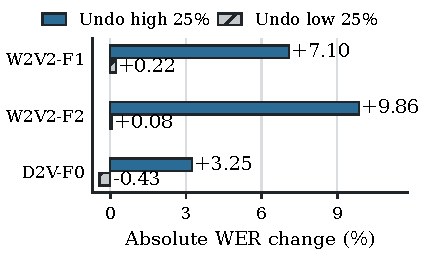
\includegraphics[width=\linewidth]{figures/deletion_effect.pdf}
\caption{WER change when the highest- or lowest-scoring quarter of fine-tuning changes is undone. Both conditions restore 256 native coordinates to the reference values and use the same adapted head. Positive values mean worse recognition.}
\label{fig:deletion}
\end{figure}

The interventions share the model, head, utterances, and coordinate count. Their contrast therefore shows non-uniform reliance on native-coordinate changes rather than a generic tolerance to removing coordinates; the training-derived ranking transfers to held-out speakers.

\subsection{Does selection follow the learned native coordinate frame?}
\label{sec:reparam}
We next test whether the concentration is tied to the coordinate system exposed by the trained head. We use the equivalent parameterization $E'=QE$, $W'_a=W_aQ^\top$, and unchanged $b_a$ as a controlled change of coordinate frame, so $W'_aE'+b_a=W_aE+b_a$. On Rel-W2V2-F0, five random bases preserve decoded predictions and WER (8.590\% dev; 10.499\% test). Native utility mass exceeds the rotated null at every top-$K$ level (Table~\ref{tab:reparam}); top-1\% Jaccard overlap is zero and top-10\% overlap is $0.058\pm0.021$. DADS concentration therefore follows the coordinate organization established at the trained encoder--head interface.

\begin{table}[t]
\centering
\caption{Rel.-F0 utility mass contained in the top native coordinates. Rotated values are mean $\pm$ SD over five equivalent orthogonal reparameterizations.}
\label{tab:reparam}
\setlength{\tabcolsep}{4pt}
\begin{tabular}{lcc}
\toprule
Top coordinates & Native & Orthogonal rotations \\
\midrule
1\%  & 7.78  & 3.37 $\pm$ 0.22 \\
5\%  & 20.23 & 12.68 $\pm$ 0.39 \\
10\% & 30.30 & 21.55 $\pm$ 0.37 \\
25\% & 50.93 & 42.38 $\pm$ 0.18 \\
\bottomrule
\end{tabular}
\end{table}

\subsection{How does calibration affect selection?}
\label{sec:robustness}
We vary the calibration size while fixing the model and head. With 128 utterances, DADS gives $13.11\pm0.13\%$ WER at 50\% and $11.11\pm0.10\%$ at 75\%, within 0.2 points of the full-set results (12.94\% and 10.96\%). Top-quarter overlap with the full ranking rises from 81.9\% at 128 utterances to 91.3\% at 512 and 94.9\% at 1,024, while WER remains similar. Thus, a small calibration sample is sufficient for useful selection.

\section{Conclusion}
\label{sec:conclusion}
DADS identifies decision-aligned native shifts: CTC sensitivity preserves recognition, reversion confirms unequal reliance, and the native-frame controls show that utility depends on the coordinate system.

% The four technical pages end here; references begin on page five.
\clearpage
\bibliographystyle{IEEEbib_initials}
\bibliography{references}
\end{document}
